\documentclass[a4paper]{article}
\usepackage[letterpaper, margin=1in]{geometry} % page format
\usepackage{listings} % this package is for including code
\usepackage{graphicx} % this package is for including figures
\usepackage{amsmath}  % this package is for math and matrices
\usepackage{amsfonts} % this package is for math fonts
\usepackage{tikz} % for drawings
\usepackage{hyperref} % for urls

\title{Homework 1}
\author{Amy Pitts}
\date{2/5/19}

\begin{document}
\lstset{language=Python}

\maketitle

\section{Problem 1.2}
Consider the perceptron in two dimensions: $h(x)=sign(w^Tx)$
where $w=[w_0,w_1,w_2]^T$ and $x=[1,x_1,x_2]^t$. 
Technically, $x$ has three coordinates, but we call this 
perception two-dimensional because the first coordinates 
is fixed at 1. \\
(a) Show that the regions on the plane where $h(x)=+1$
and $h(x)=-1$ are separated by a line. If we express
this line by the equation $x_2=ax_1+b$ what are 
the slope $a$ and intercept $b$ in terms of $w_0,w_1,x_2$? \\
\indent \textbf{Solution:} If we have $h(x)=1$ and $h(x)=-1$ this 
implies that for $h(x)=1$ we have $w^Tx>0$ and with $h(x)=-1$ we 
have $w^Tx<0$ so the separation between the two is just the 
x-axis or when $w^Tx=0$. \\
For the equation $x_2=ax_1+b$ we have that $a= -\frac{w_1}{w_2}$ and $b=-\frac{w_0}{w_2}$

(b) Draw a picture for the cases $w=[1,2,3]^T$ and $w=-[1,2,3]^T$. \\
In more than two dimensions, the $+1$ and $-1$ regions are
separated by a hyperplane, the generalization of a line. \\
\indent \textbf{Solution:} \\
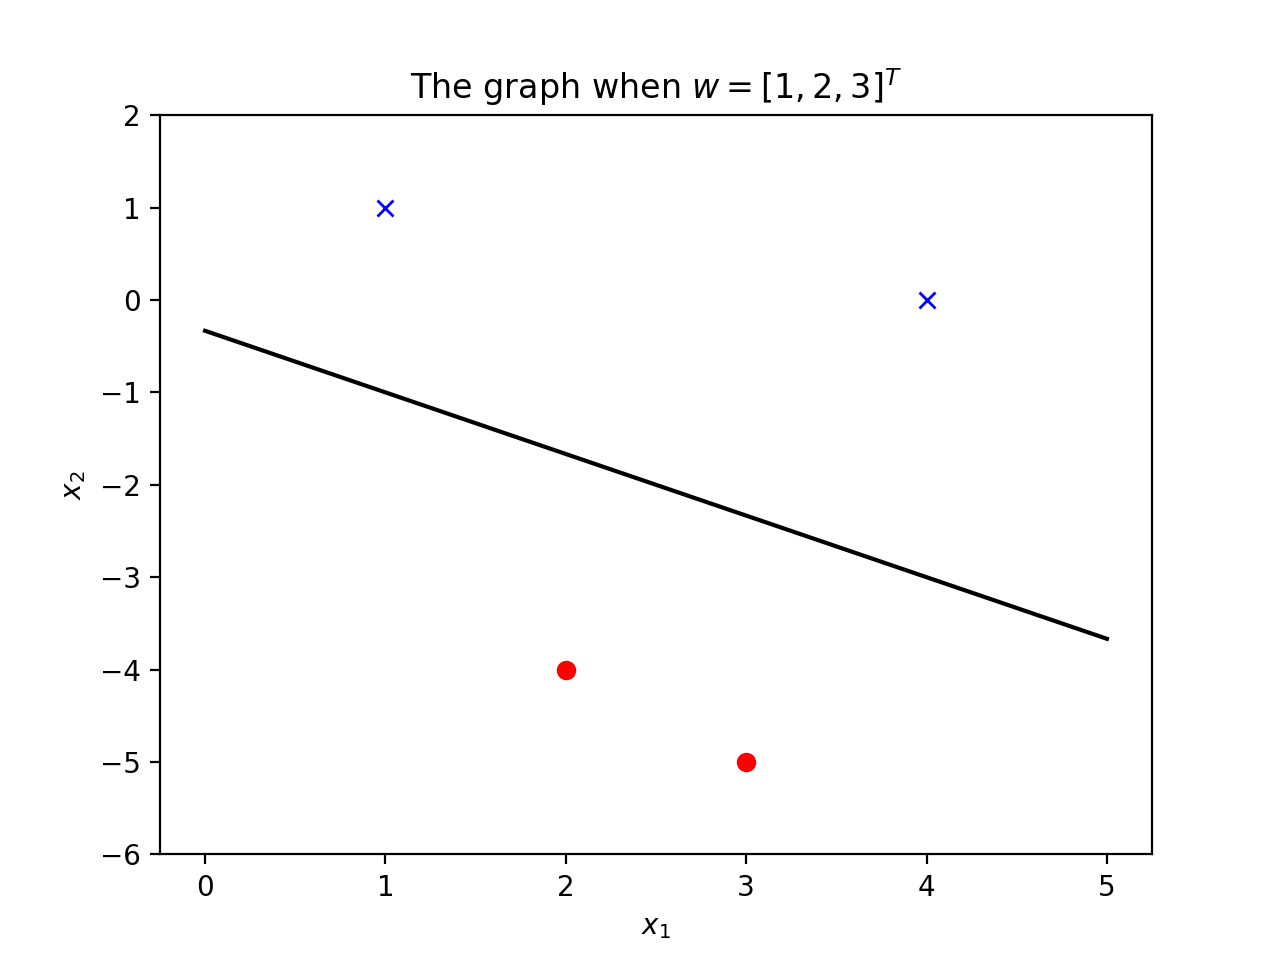
\includegraphics[width=85mm]{positive.png}
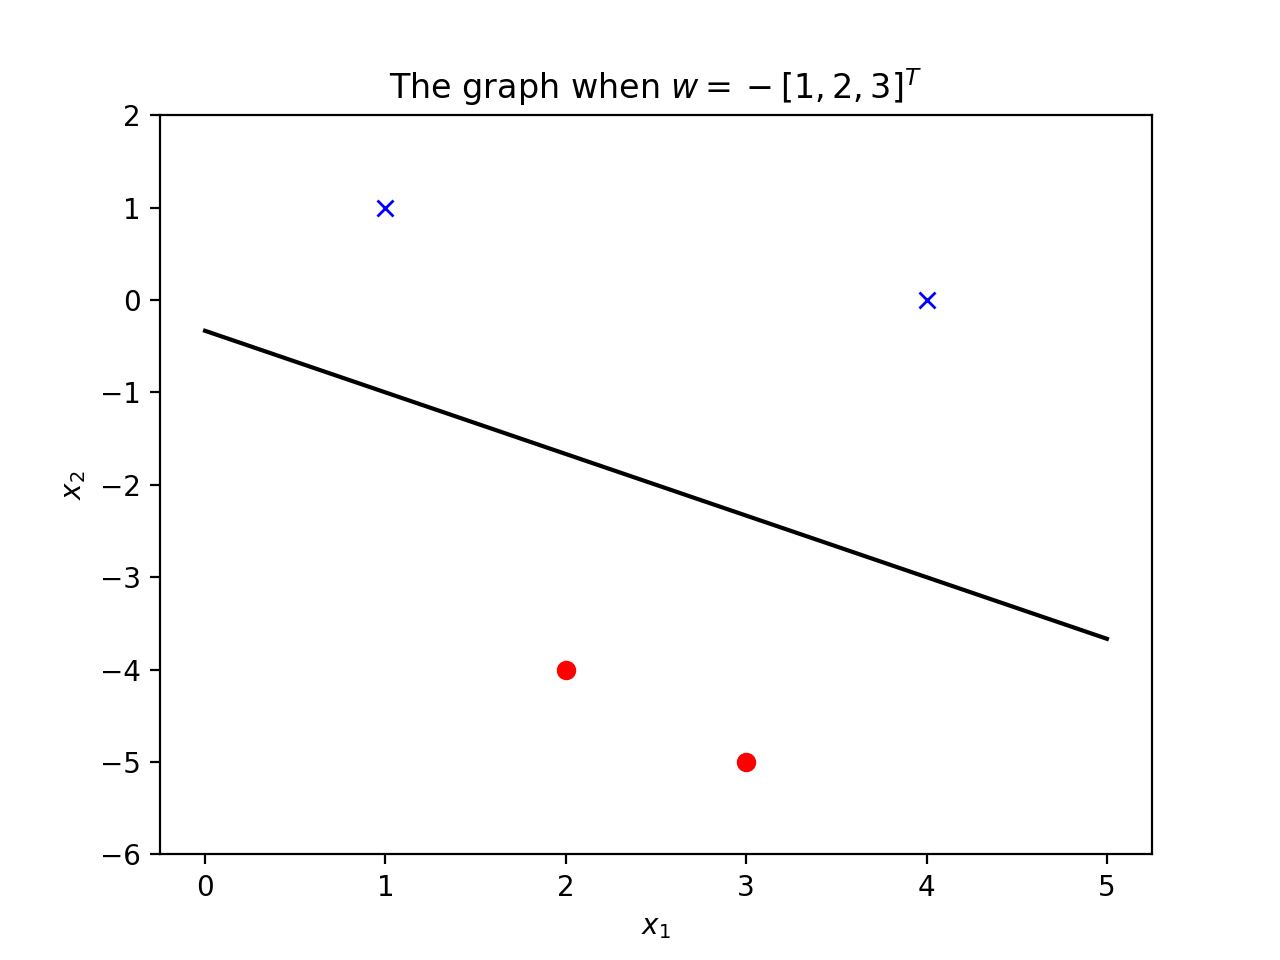
\includegraphics[width=85mm]{negative.png} \\
\lstinputlisting[language=Python,frame=single]{plotting_practice.py}


\section{Problem 1.4}
In Exercise 1.4 we use an artificial data set to study the 
perceptron learning algorithm. This problem leads you to explore the algorithm
further with data sets of different sizes and dimensions. \\
\indent For the following question I will be using and modifying 
this code: 
\lstinputlisting[language=Python,frame=single]{plotP.py}
\indent \textbf{(a):} Generate a linearly separable data set of 
size 20 as indicated in Exercise 1.4. Plot the examples
$\{(x_n,y_n)\}$ as well as the target function $f$ on a plane. Be sure
to mark the examples from different classes differently, 
and add labels to the axes of the plot. \\
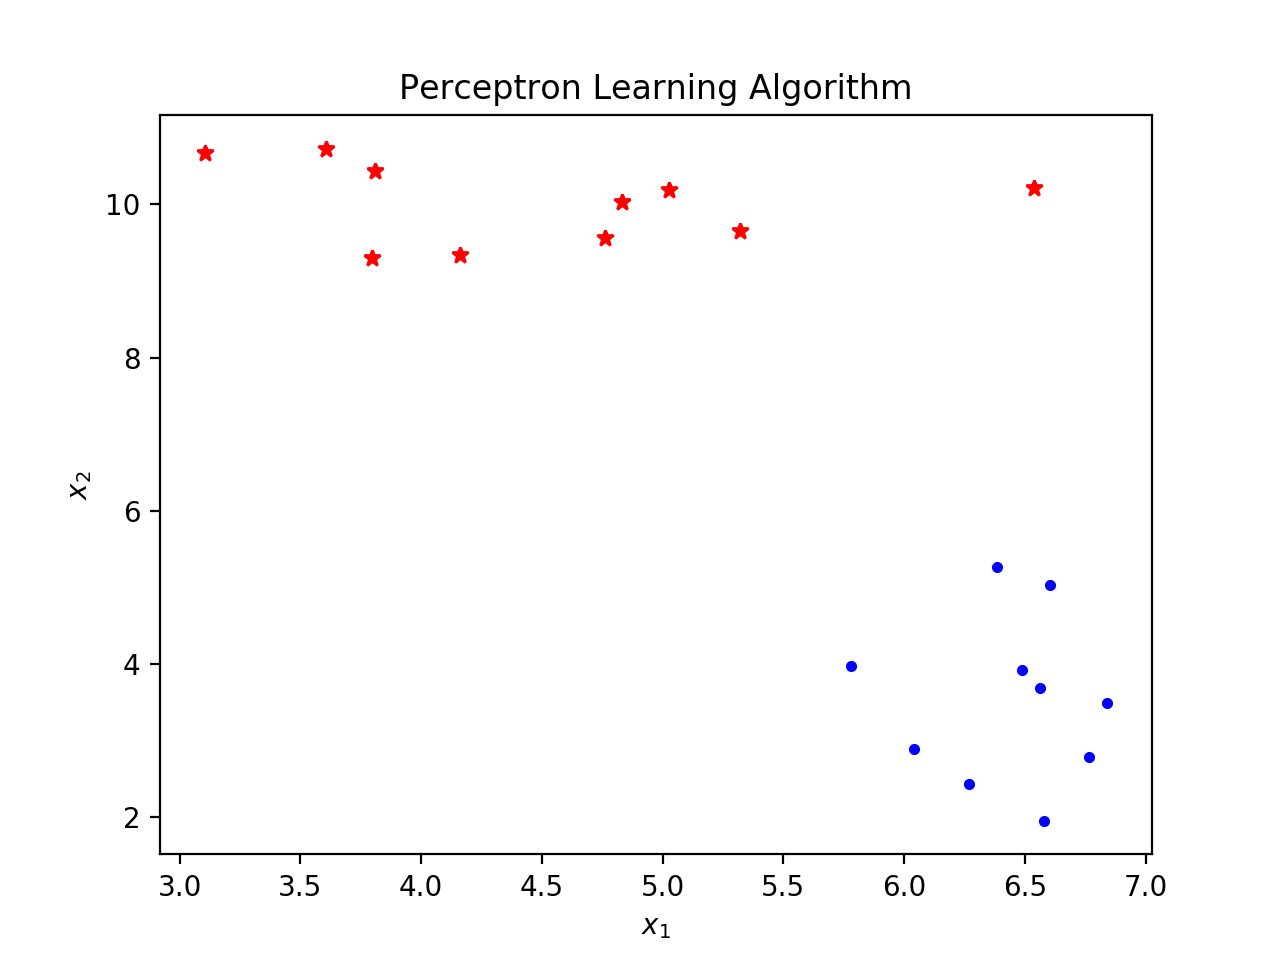
\includegraphics[width=85mm]{a_1.png} 
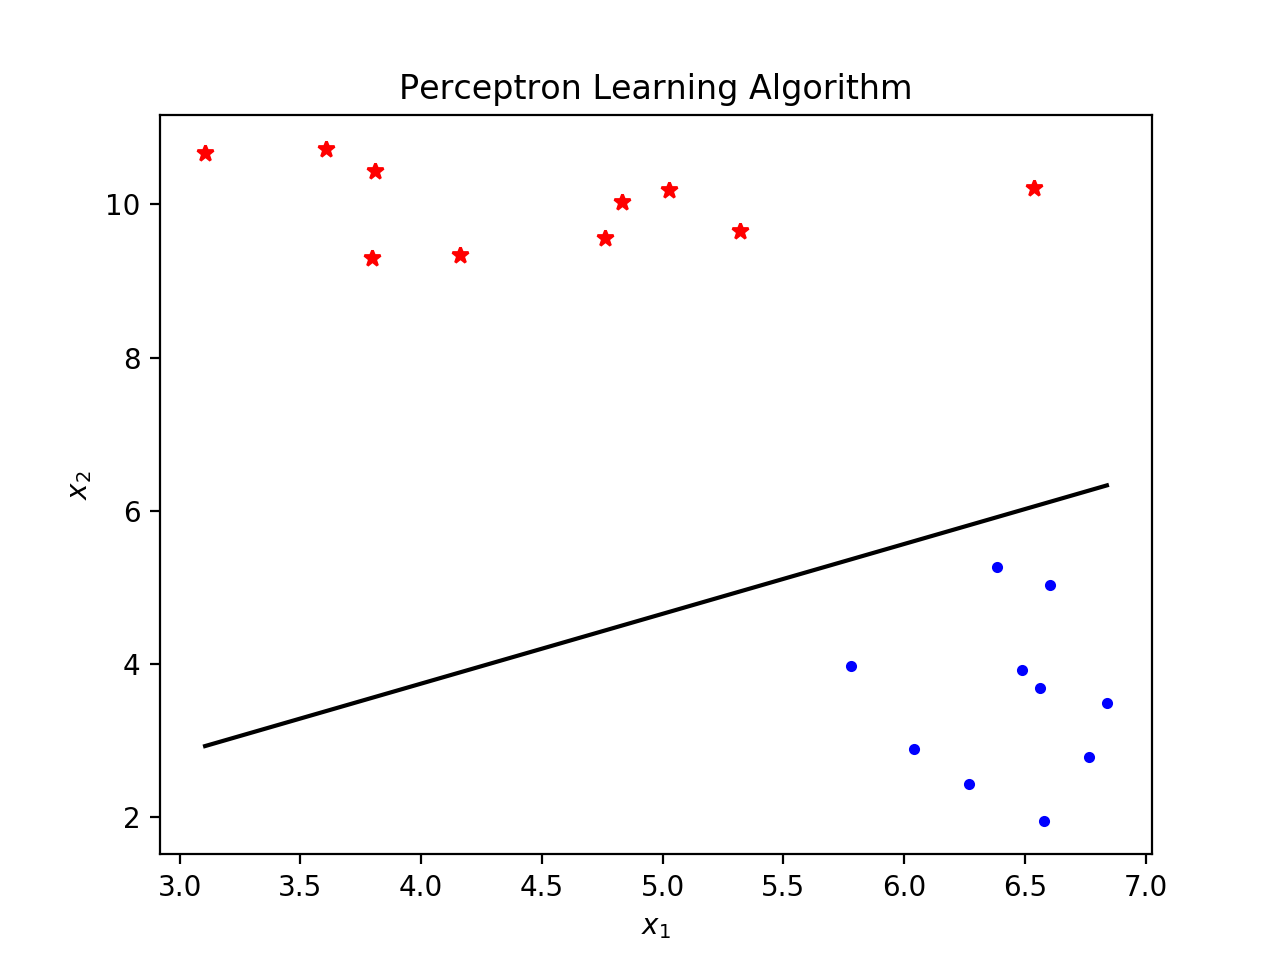
\includegraphics[width=85mm]{a_2.png} \\
The program took 5 iterations to properly split up the two groups. \\


\indent \textbf{(b):} Run the perceptron learning algorithm on 
the data set above. Report the number of updates that the algorithm
takes before converging. Plot the examples $\{(x_n,y_n)\}$, and the
final hypothesis $g$ in the same figure. Comment on whether $f$ is 
close to $g$. \\
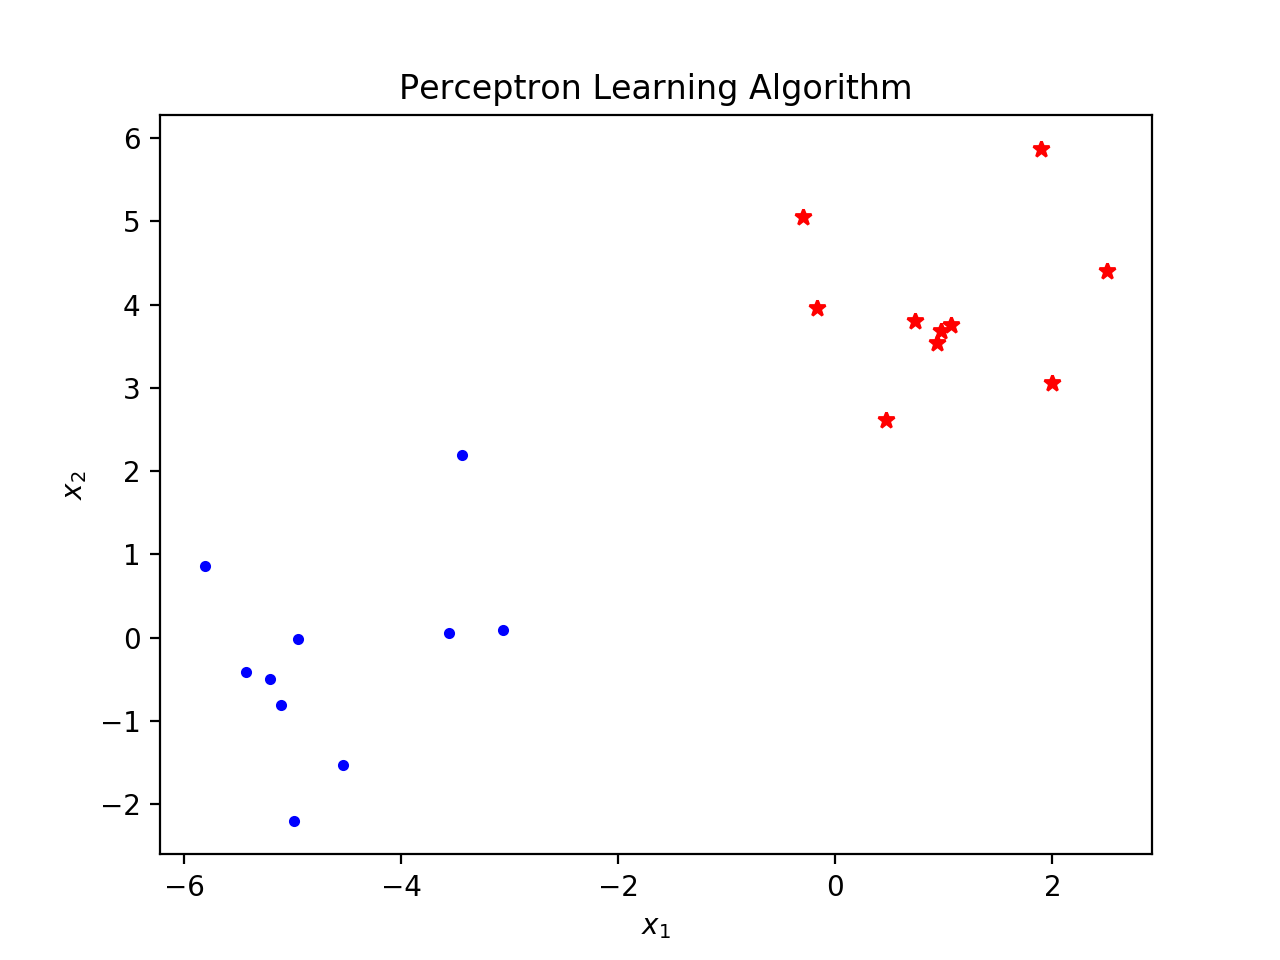
\includegraphics[width=85mm]{b_1.png} 
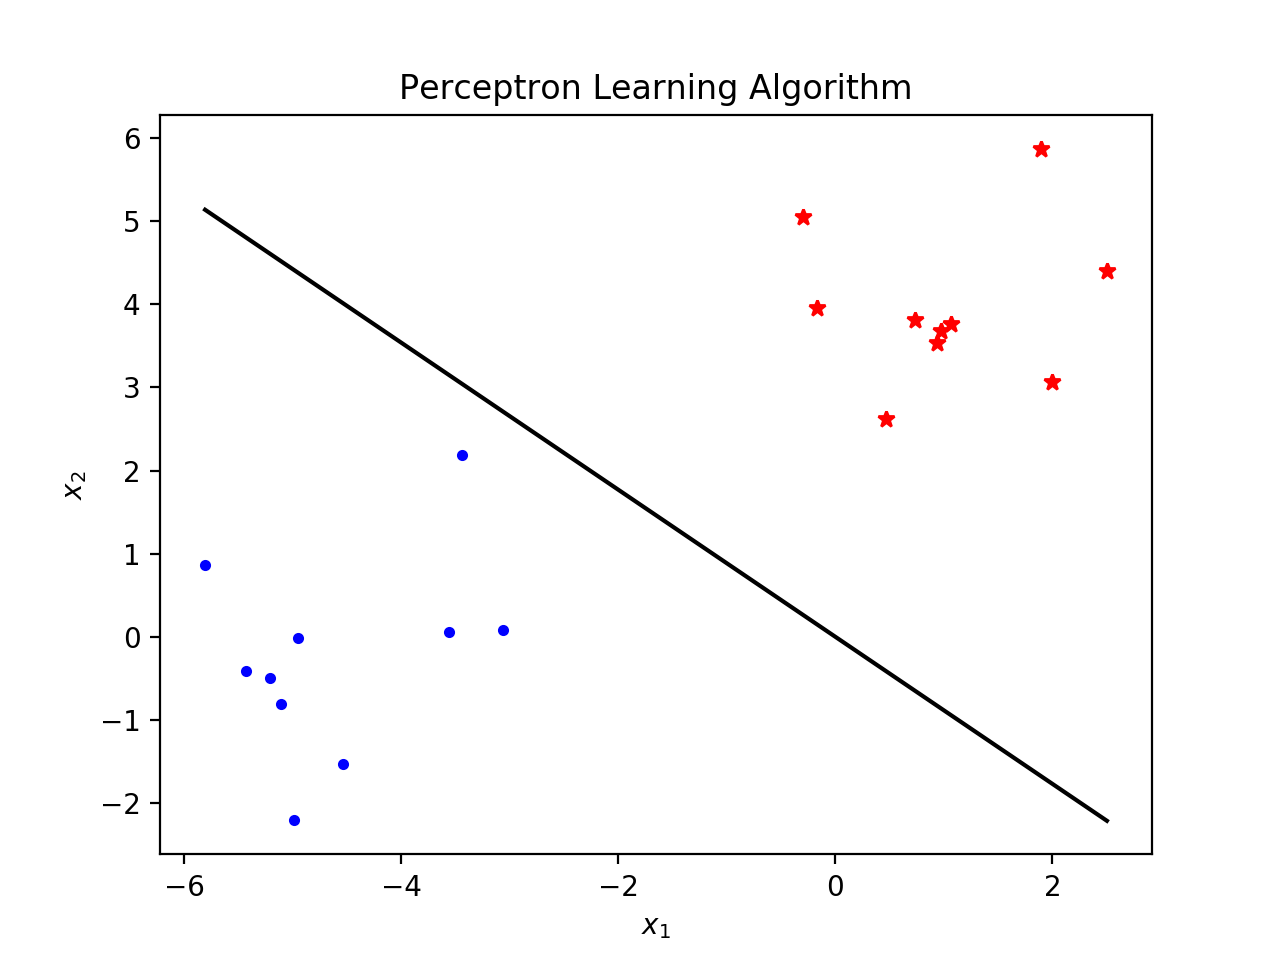
\includegraphics[width=85mm]{b_2.png} \\
The program took 2 iterations to properly split up the two groups.
We are unable to tell if $f$ is close to $g$ because we do not know 
what $f$ is. \\ 

\indent \textbf{(c):} Repeat everything in (b) with another randomly
generated data set of size 20. Compare your results with (b). \\
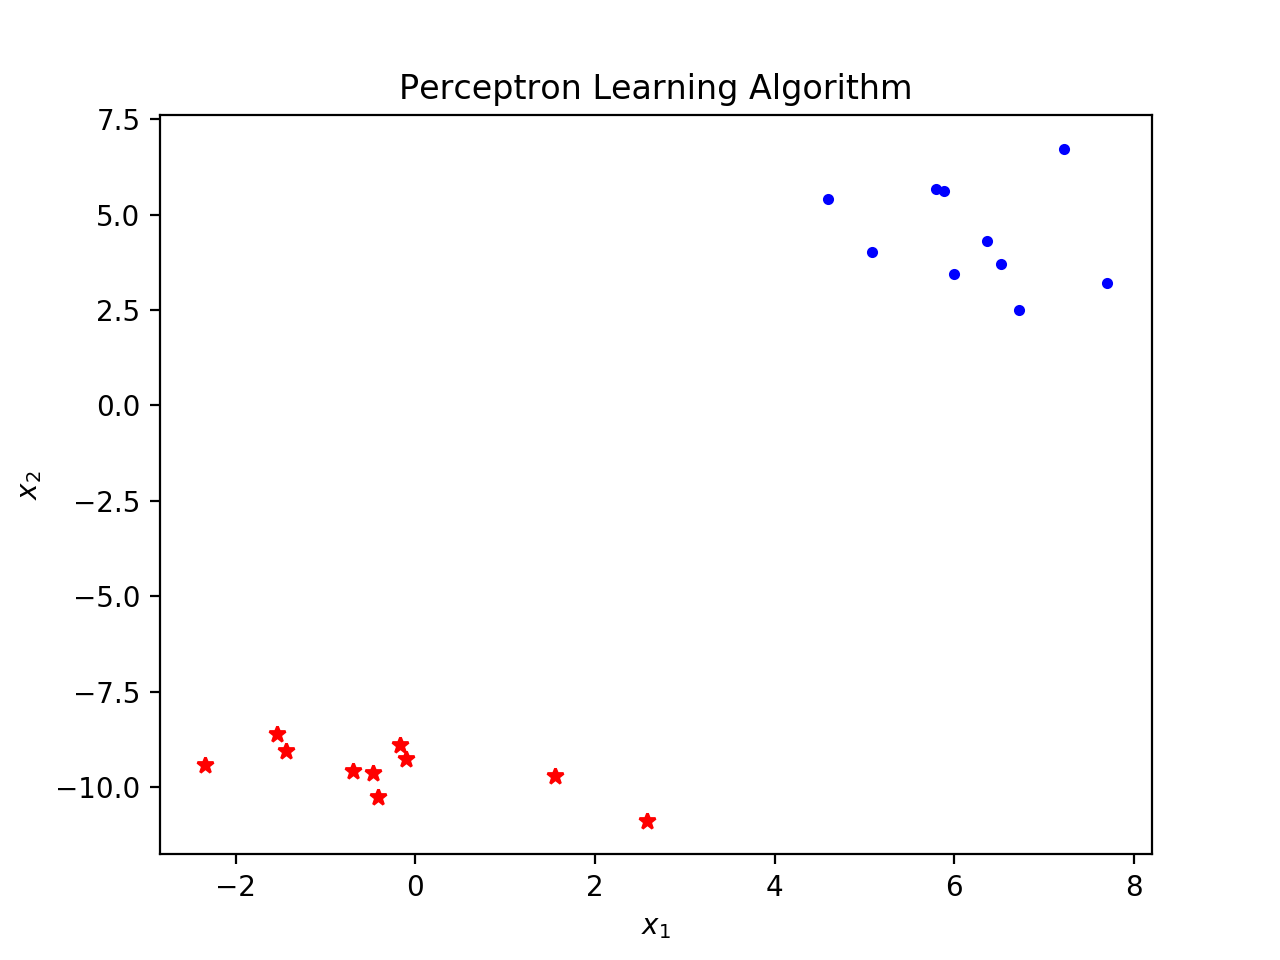
\includegraphics[width=85mm]{c_1.png} 
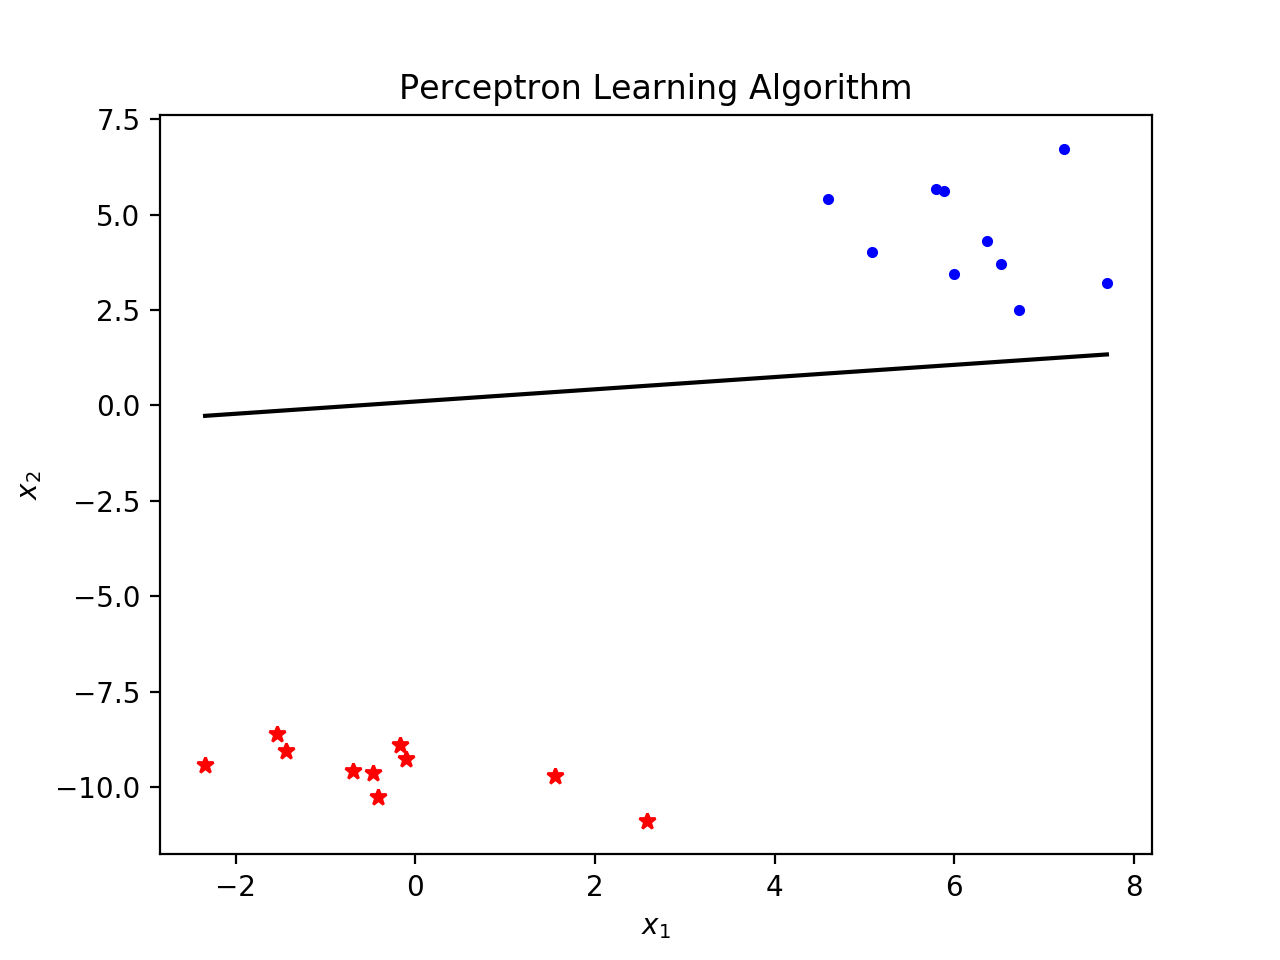
\includegraphics[width=85mm]{c_2.png} \\
The program took 1 iteration to properly split up the two groups.
We are unable to tell if $f$ is close to $g$ because we do not know 
what $f$ is. \\ 

\indent \textbf{(d):} Repeat everything in (b) with another randomly
generated data set of size 100. Compare your results with (b). \\
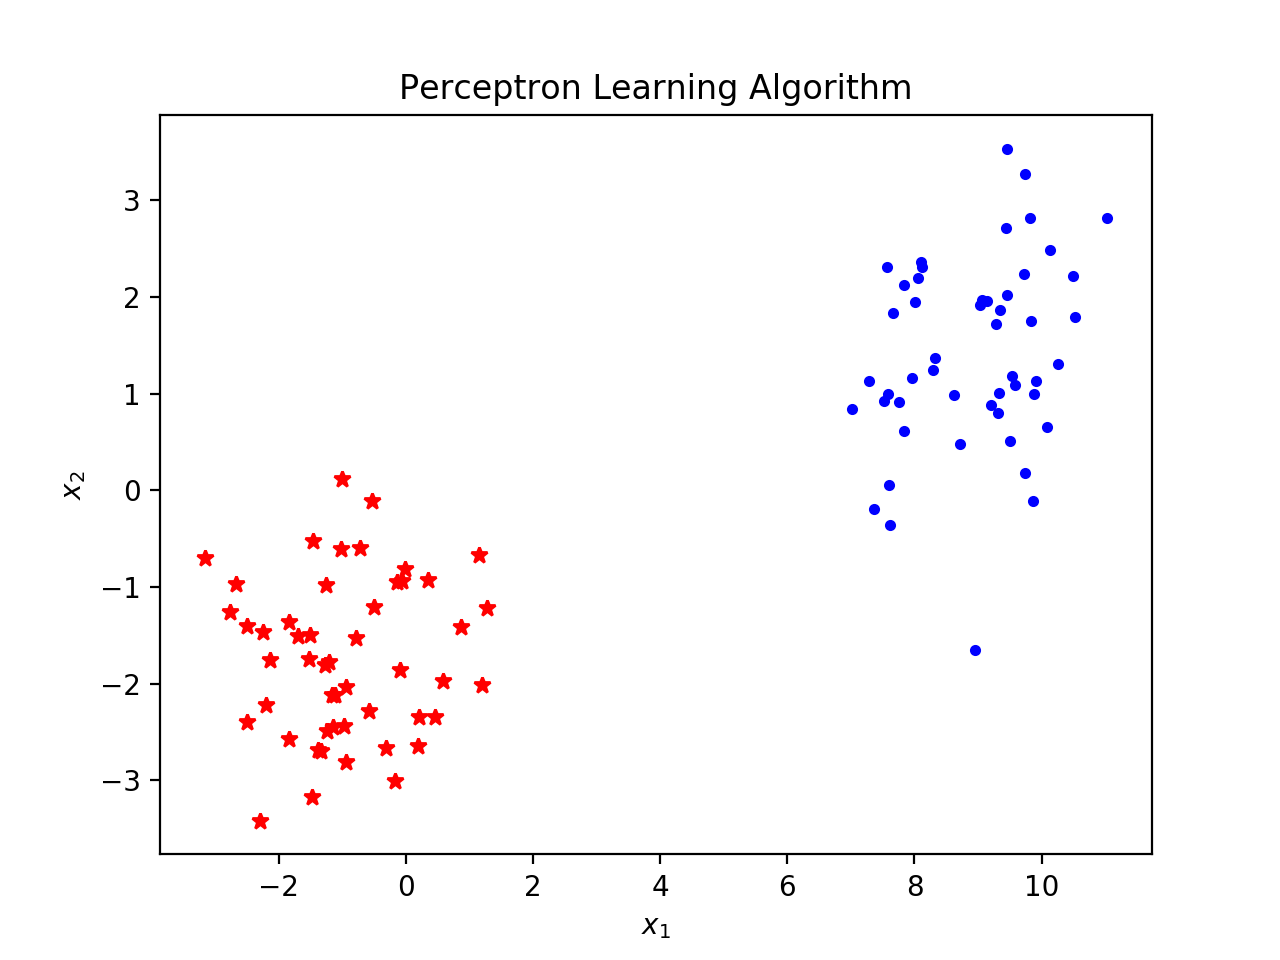
\includegraphics[width=85mm]{d_1.png} 
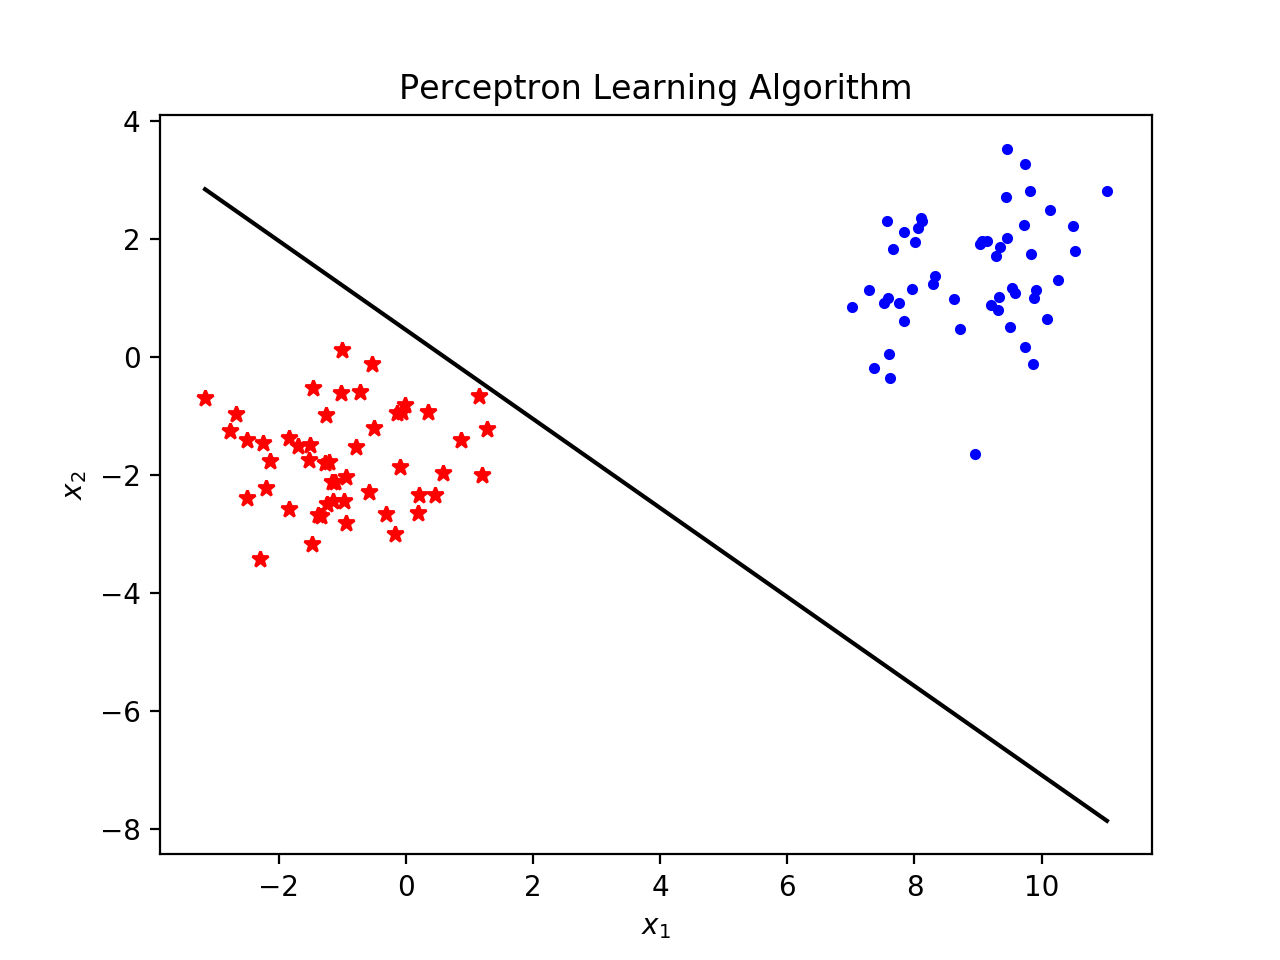
\includegraphics[width=85mm]{d_2.png} \\
The program took 5 iteration to properly split up the two groups.\\

\indent \textbf{(e):} Repeat everything in (b) with another randomly
generated data set of size 1,000. Compare your results with (b). \\
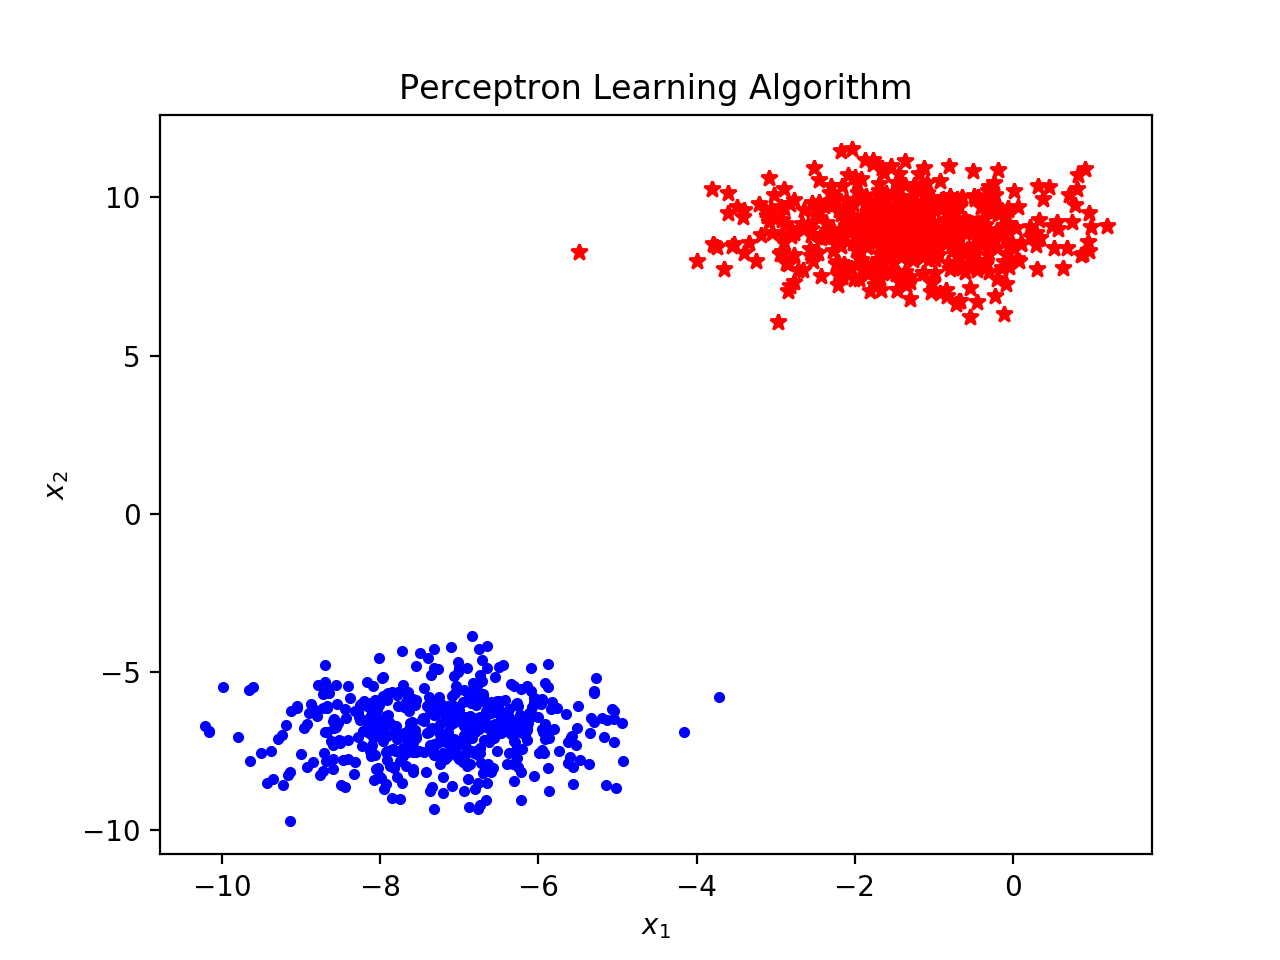
\includegraphics[width=85mm]{e_1.png} 
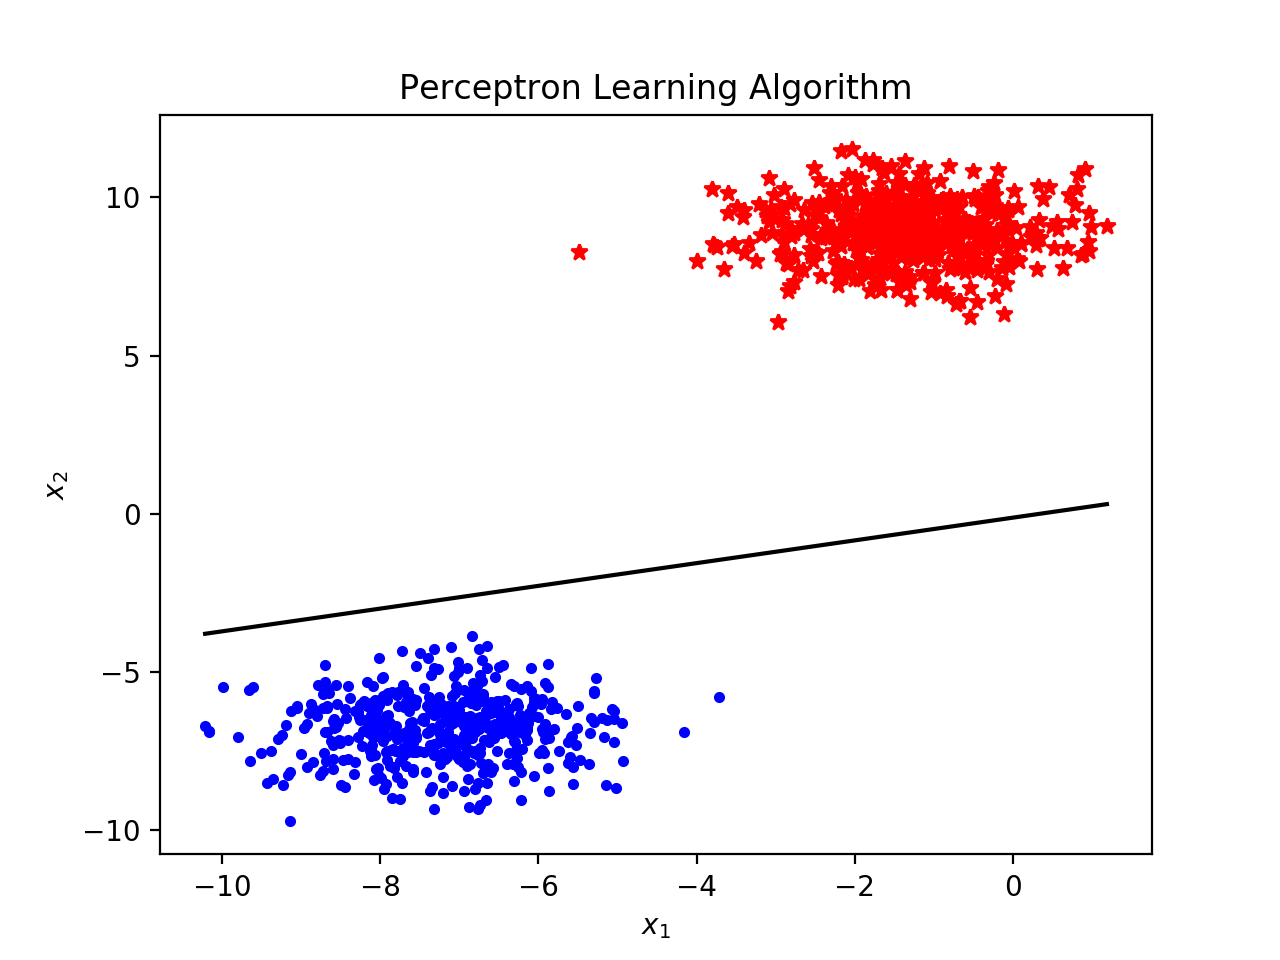
\includegraphics[width=85mm]{e_2.png} \\
The program took 1 iteration to properly split up the two groups.
I thought it was going to take more iterations but the 
data generator is making perfectly separated groups making 
it super easy to separate. Also, after running the program
a couple of times to see what happens I found that I either get 
stuck in a loop of never being able to find the perfect line
or the groups are easily separated and it take 1 to 2 iterations. 
\\


\indent \textbf{(f):} Modify the algorithm such that it takes 
$x_n \in \mathbb{R}^{10}$ instead of $\mathbb{R}^2$. Randomly generate
a linearly separable data set of size 1,000 with $x_n \in \mathbb{R}^{10}$
and feed the data set to the algorithm. How many updates does the 
algorithm take to converge? \\
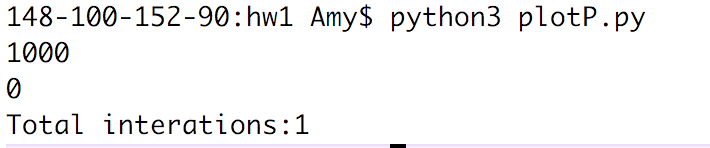
\includegraphics[width=85mm]{f.png} \\
The algorithm took one update to converge. \\


\indent \textbf{(g):} Repeat the algorithm on the same data set as (f)
for 100 experiments. In the iterations of each experiment, pick 
$x(t)$ randomly instead of deterministically. Plot a histogram
for the number of updates that the algorithm take to converge. \\ 
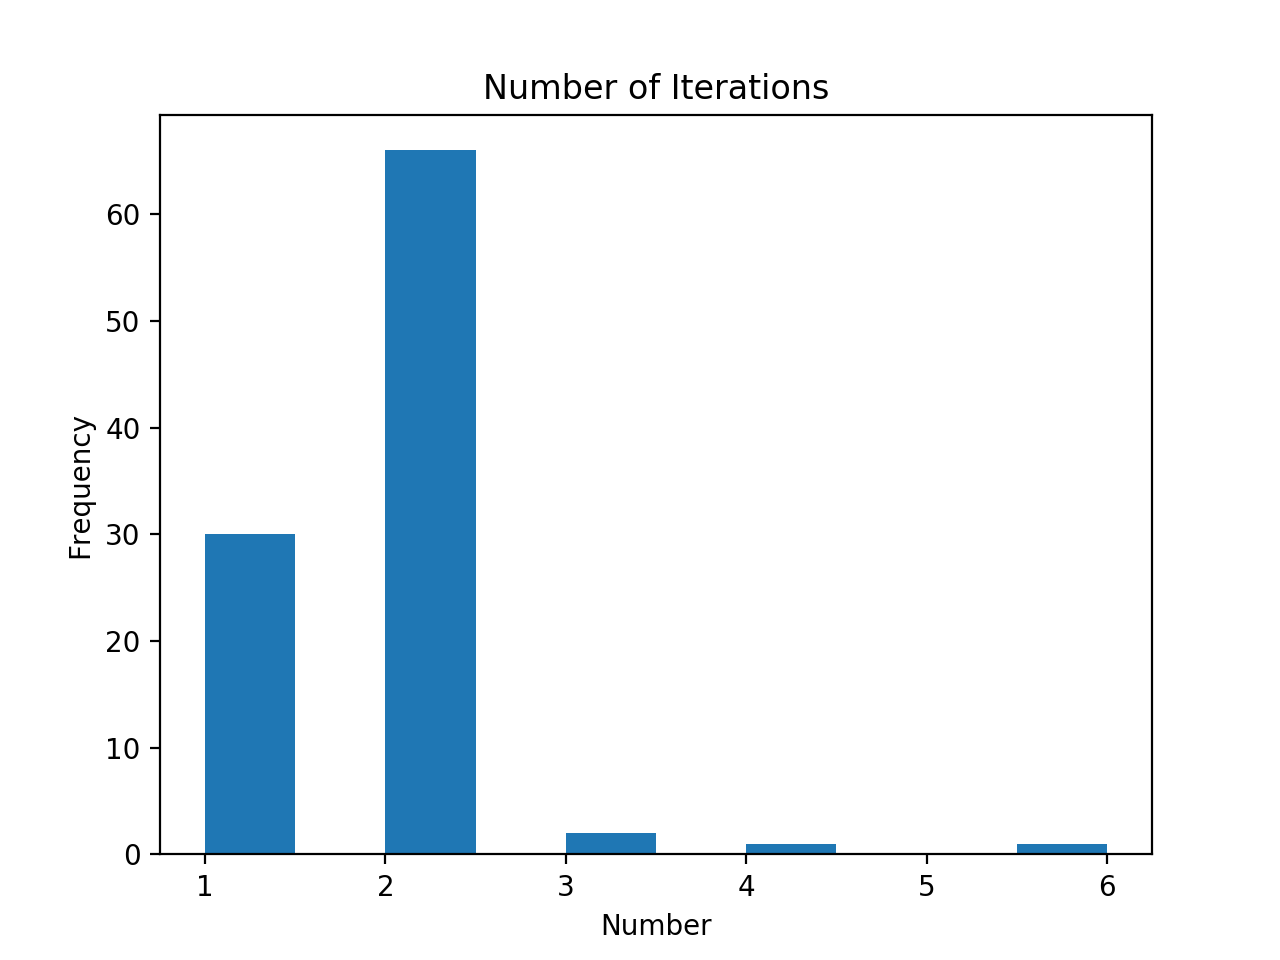
\includegraphics[width=150mm]{g.png} \\
\lstinputlisting[language=Python,frame=single]{10_dims.py}


\indent \textbf{(h):} Summarize your conclusions with respect to 
accuracy and running time as a function of $N$ and $d$. \\

I found that the generated data if broken up takes about 1 to 
2 iterations to properly split the data. However, 
when there were only two dimensions there was a more 
likely chance that a data set was generated that was not 
able to be split up resulting in an endless loop. 
Running the 10-dimensional data set there was less of a 
chance that the data would not be able to be split. 
Also when $N$ was increased there was a higher chance 
that a data set was produced that was not able to be split 
by a line. I wonder what would happen if we used a 
different data generator. 

\end{document}
